%
% labor.tex -- graphische Darstellung des Labor-Experiments
%
% (c) 2017 Prof Dr Andreas Müller, Hochschule Rapperswil
%
\documentclass[tikz]{standalone}
\usepackage{times}
\usepackage{txfonts}
\usepackage{fp}
\usepackage{ifthen}
\usepackage[utf8]{inputenc}
\usetikzlibrary{arrows,intersections}
\usetikzlibrary{fixedpointarithmetic}
\begin{document}
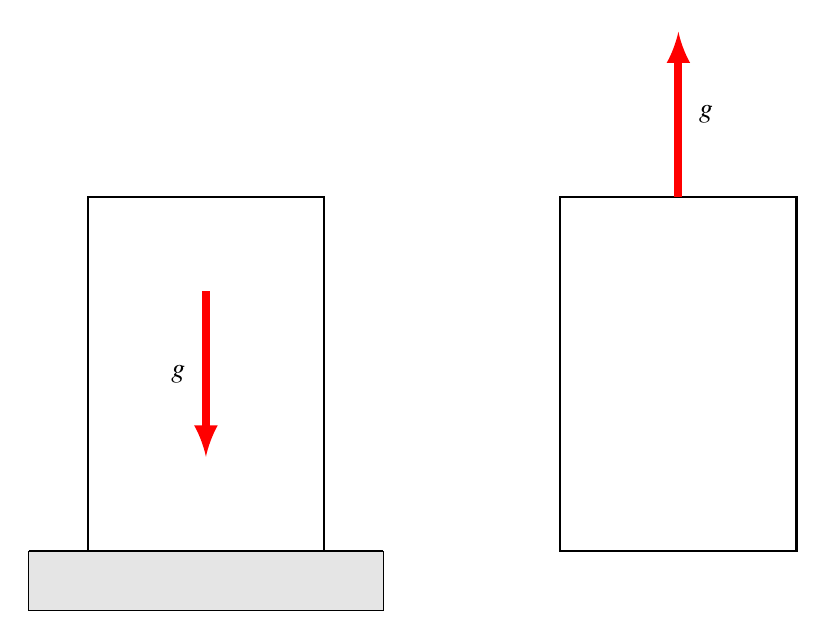
\begin{tikzpicture}[>=latex, thick, scale=1.5]

\draw (-3,0)--(-1,0)--(-1,3)--(-3,3)--cycle;
\draw (-3.5,0)--(-0.5,0);
\draw[->,red,line width=1mm] (-2,2.2)--(-2,0.8);
\node[red,label={left:$g$}] at (-2,1.5) {};

\draw[fill=gray!20,line width=0] (-3.5,0)--(-0.5,0)--(-0.5,-0.5)--(-3.5,-0.5)--cycle;

\draw (3,0)--(1,0)--(1,3)--(3,3)--cycle;
\draw[->,red,line width=1mm] (2,3)--(2,4.4);
\node[red,label={right:$g$}] at (2,3.7) {};

\end{tikzpicture}
\end{document}
